\documentclass{cernatsnote}
\usepackage{physics}
\usepackage{tcolorbox}
\tcbuselibrary{skins}
\usepackage{lipsum}
\usepackage{mathtools}
\usepackage{amsfonts}
\usepackage[colorinlistoftodos]{todonotes}
\usepackage{placeins}
\usepackage{amsmath}
\usepackage{physics}
\usepackage{tcolorbox}
\tcbuselibrary{skins}
\usepackage{lipsum}
\usepackage{amsmath}
\usepackage[T1]{fontenc}
\usepackage{graphicx, subfigure}
\usepackage{fancyhdr}
\usepackage{lmodern}
\usepackage{color}
\usepackage{transparent}
\usepackage{amsfonts}
\usepackage{mathtools}
\usepackage{tikz}
\usetikzlibrary{positioning}
\usepackage{pgfplots}
\pgfplotsset{compat=1.10}
\usepackage{textcomp}
\usepackage{float}
\usepackage{adjustbox} % Used to constrain images to a maximum size 
\usepackage{color} % Allow colors to be defined
\usepackage{enumerate} % Needed for markdown enumerations to work
\usepackage{geometry} % Used to adjust the document margins
\usepackage{amsmath} % Equations
\usepackage{amssymb}
\usepackage{fancyvrb} % verbatim replacement that allows latex
\usepackage{grffile} % extends the file name processing of package graphics 
                         % to support a larger range 
    % The hyperref package gives us a pdf with properly built
    % internal navigation ('pdf bookmarks' for the table of contents,
    % internal cross-reference links, web links for URLs, etc.)
\usepackage{hyperref}
\usepackage{longtable} % longtable support required by pandoc >1.10
\usepackage{tabularx}
\usepackage{epigraph}
\usepackage{quotchap}
\usepackage{lscape}
\usepackage{enumerate}
\usepackage{xpatch}
\usepackage{titletoc}
\usepackage{float}	
\usepackage{xparse}
\NewDocumentCommand{\DIV}{om}{%
  \IfValueT{#1}{\setcounter{#2}{\numexpr#1-1\relax}}%
  \csname #2\endcsname
}

\newtcolorbox{mybox}[3][]
{
  colframe = #2!25,
  colback  = #2!10,
  coltitle = #2!20!black,  
  title    = {#3},
  #1,
}

%\renewcommand{\thesubsection}{\thesection.\alph{subsection}}


\title{Computational Physics – Exercise 7}
\author{Pugazharasu Anancia Devaneyan, Rishi Kumar Senthil Kumar}
\email{\href{pugs@uni-bonn.de}{pugs@uni-bonn.de}, \href{s6risent@uni-bonn.de}{s6risent@uni-bonn.de}}
\date{\today}

\begin{document}
\maketitle

%\begin{abstract}
%This document summarizes ideas from Group theory and representation theory that are vital for the upcoming seminar.
%\end{abstract}
%\\ \\ \\ 

%\begingroup
%\color{black}
%\tableofcontents
%\endgroup

%\section*{Test}
%\section*{Simulation of the 1-D Ising model}
\section{Coding the Swendsen-Wang Algorithm}
We coded the Swendsen-Wang Algorithm, it can be found at \cite{github}.
\section{Computing observables}
\begin{figure}[H]
    \centering
    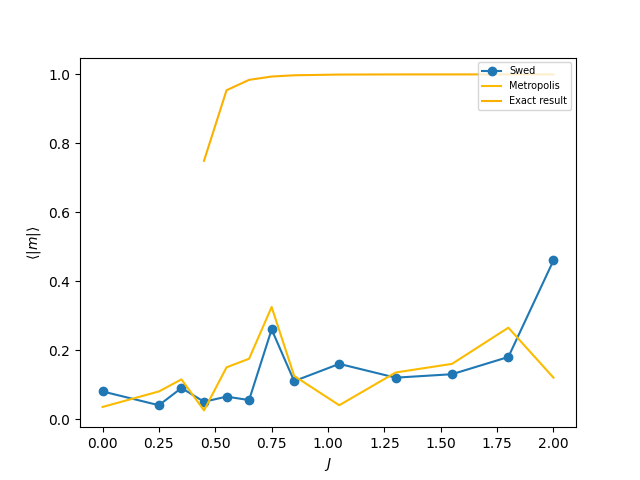
\includegraphics[scale = 0.5]{images/m_v_j.png}
    \caption{A plot of $\expval{|m|}$ vs $J$ for the exact solution and different algorithms}
    \label{fig:my_label}
\end{figure}

\begin{figure}[H]
    \centering
    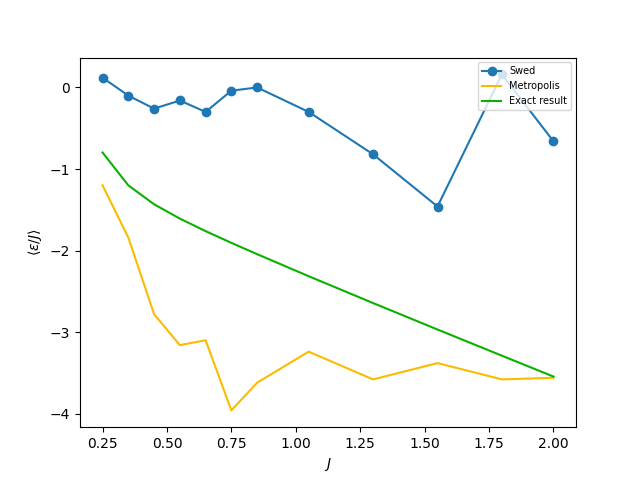
\includegraphics[scale = 0.5]{images/e_v_j.png}
    \caption{A plot of $\expval{\epsilon/J}$ vs $J$ for the exact solution and different algorithms}
    \label{fig:my_label}
\end{figure}
\section{The Monte Carlo history of $m$}
-
\section{Calculating the autocorrelation time}
-
\section{Comparing dynamical exponents}
-
\bibliographystyle{abbrv}
\bibliography{Bibliography.bib}
\end{document}